\subsection{Документ "<Установка цен номенклатуры контрагентов">}
\subsubsection{Описание работы с документом ,,Установка цен номенклатуры контрагентов''}
\begin{itemize}	
	 \item 
\includegraphics[width=0.02\linewidth]{images/doc} Создан новый документ "<Установка цен номенклатуры контрагентов">      	
%	\item \todo[inline, color=blue!40]{Добавить путь к документу в интерфейсе.}%  
	\item Документ находится в разделе \menu[,]{Маркетинг, Ценообразование, ...}
	\item Открывается журнал документов
	Рис.~\ref{ris:19.jpg}	
\begin{figure}[H]
	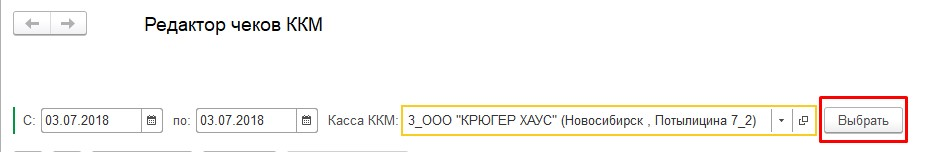
\includegraphics[width=0.8\textwidth]{19.jpg}
	\caption{Документы ,,Установка цен номенклатуры контрагентов''.}
	\label{ris:19.jpg}
\end{figure}
	Новый документ можно создать используя кнопку \keys{Создать}:
	Рис.~\ref{ris:20.jpg}	
\begin{figure}[H]
	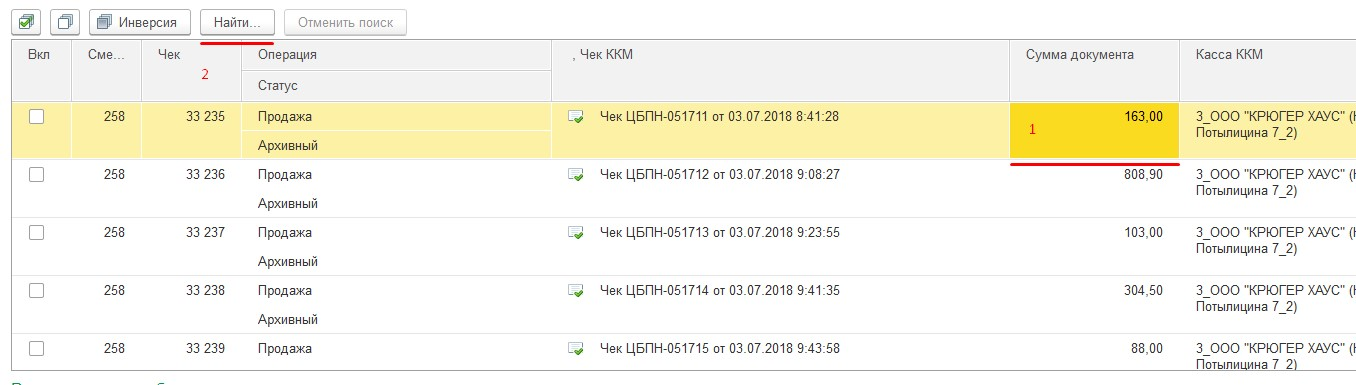
\includegraphics[width=0.8\textwidth]{20.jpg}
	\caption{Новый документ ,,Установка цен номенклатуры контрагентов''.}
	\label{ris:20.jpg}
\end{figure}
	\item Порядок создания нового документа
	\begin{enumerate}	
		\item Выбор контрагента
		\begin{itemize}		
				\item При выборе контрагента открывается вкладка с существующими ценами контрагента.
		\begin{figure}[H]
			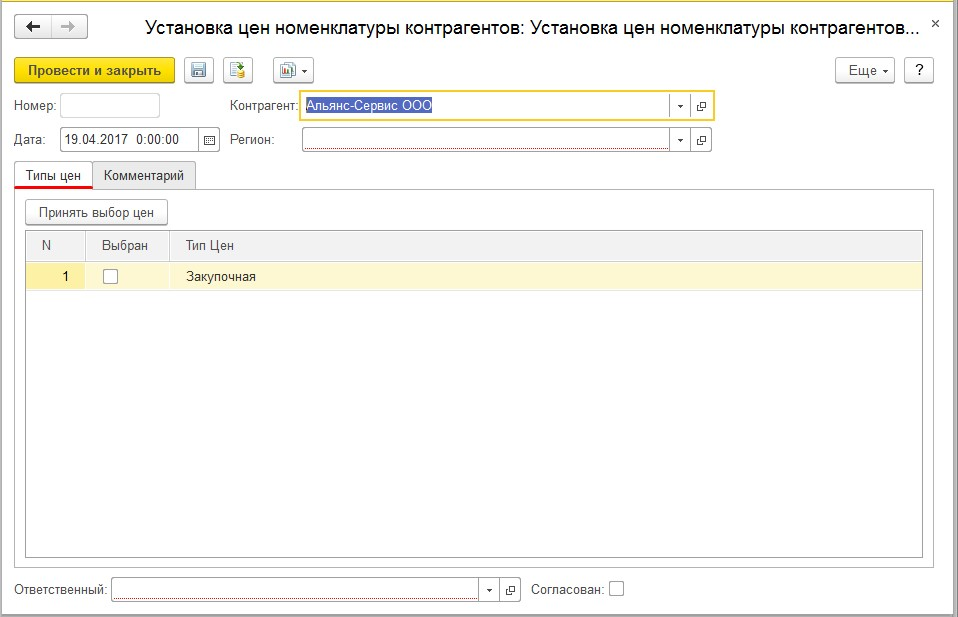
\includegraphics[width=0.8\textwidth]{21.jpg}
			\caption{Цены номенклатуры контрагентов.}
			\label{ris:21.jpg}
		\end{figure}		
			\item Необходимо в колонке "<Выбран"> отметить интересующие типы цены и нажать кнопку \keys{Принять выбор цен}.
		\begin{figure}[H]
			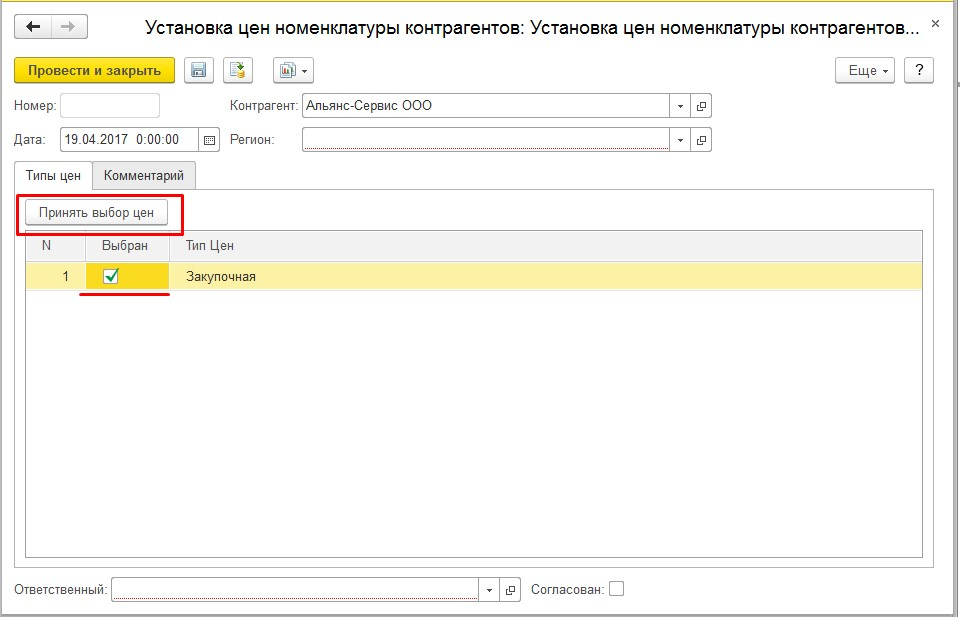
\includegraphics[width=0.8\textwidth]{22.jpg}
			\caption{Выбрать типы цен.}
			\label{ris:22.jpg}
		\end{figure}		
		\end{itemize}	
		Документ возвращается в табличную часть "<Товары">, появляются дополнительные колонки согласно выбранным типам цен.
		\begin{figure}[H]
			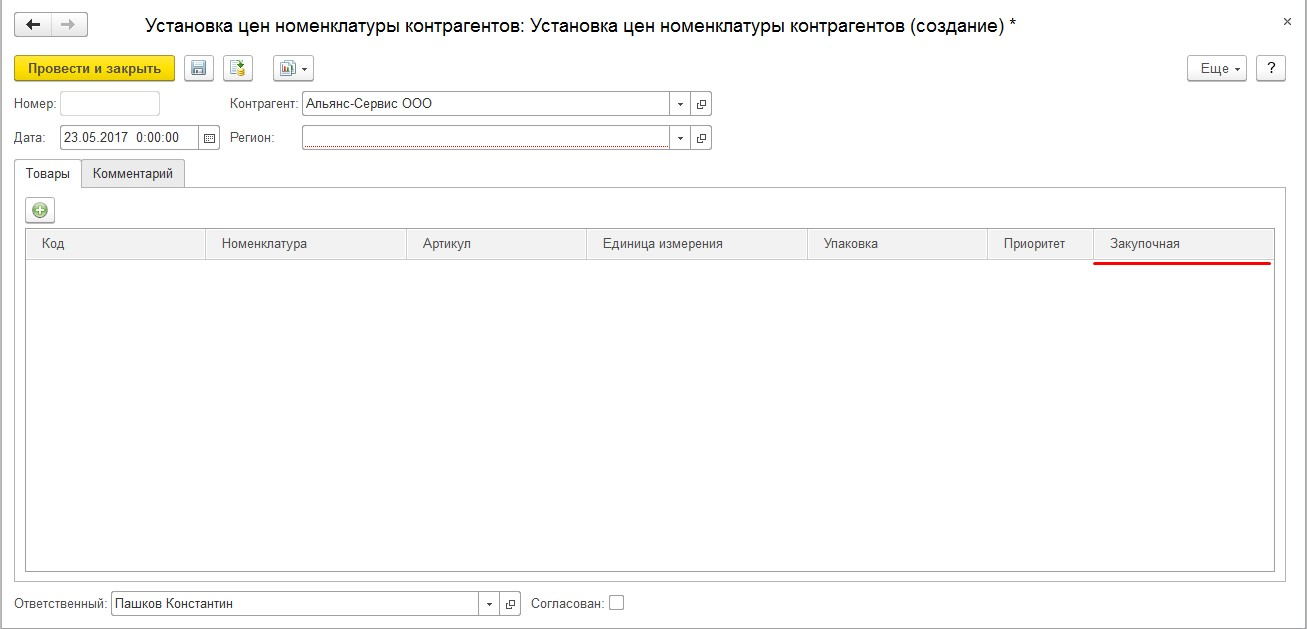
\includegraphics[width=0.8\textwidth]{23.jpg}
			\caption{Новые колонки.}
			\label{ris:23.jpg}
		\end{figure}		
		
		\item Выбор региона для которого устанавливаются цены.
		\begin{figure}[H]
			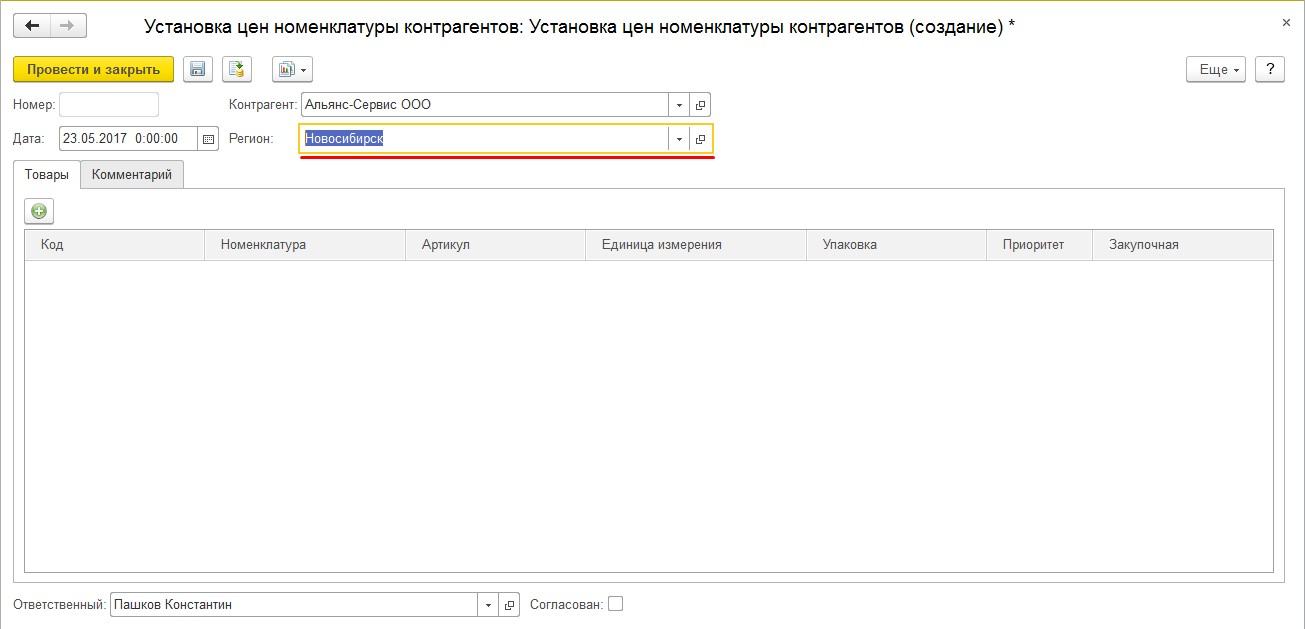
\includegraphics[width=0.8\textwidth]{25.jpg}
			\caption{Регион.}
			\label{ris:25.jpg}
		\end{figure}		
		\item Подбор номенклатуры в используя кнопку 
\includegraphics[width=0.02\linewidth]{images/new}  "<Добавить">.
		\begin{figure}[H]
			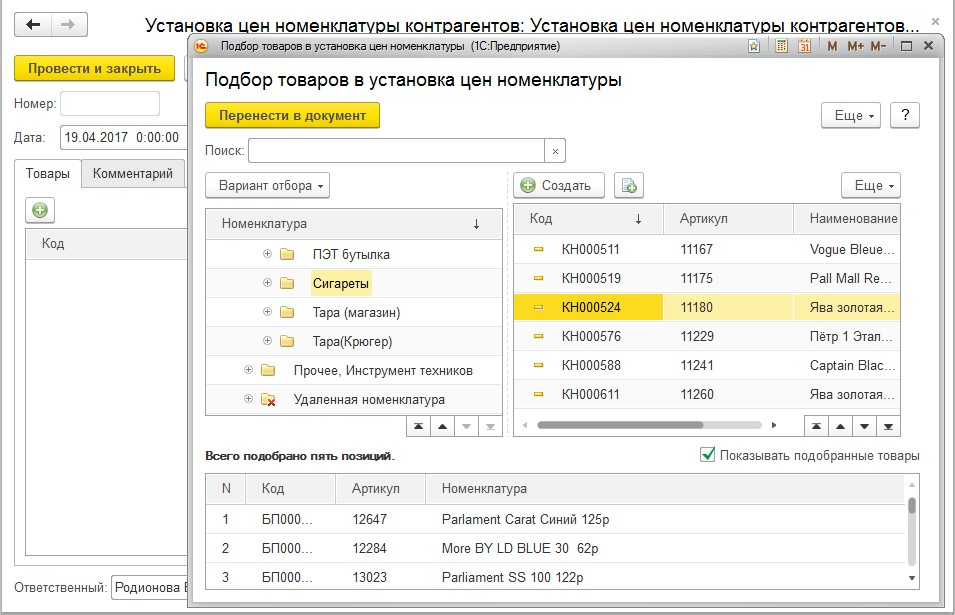
\includegraphics[width=0.8\textwidth]{24.jpg}
			\caption{Подбор номенклатуры.}
			\label{ris:24.jpg}
		\end{figure}		
		\item Теперь нужно установить цены для каждой позиции.
		 \begin{figure}[H]
		 	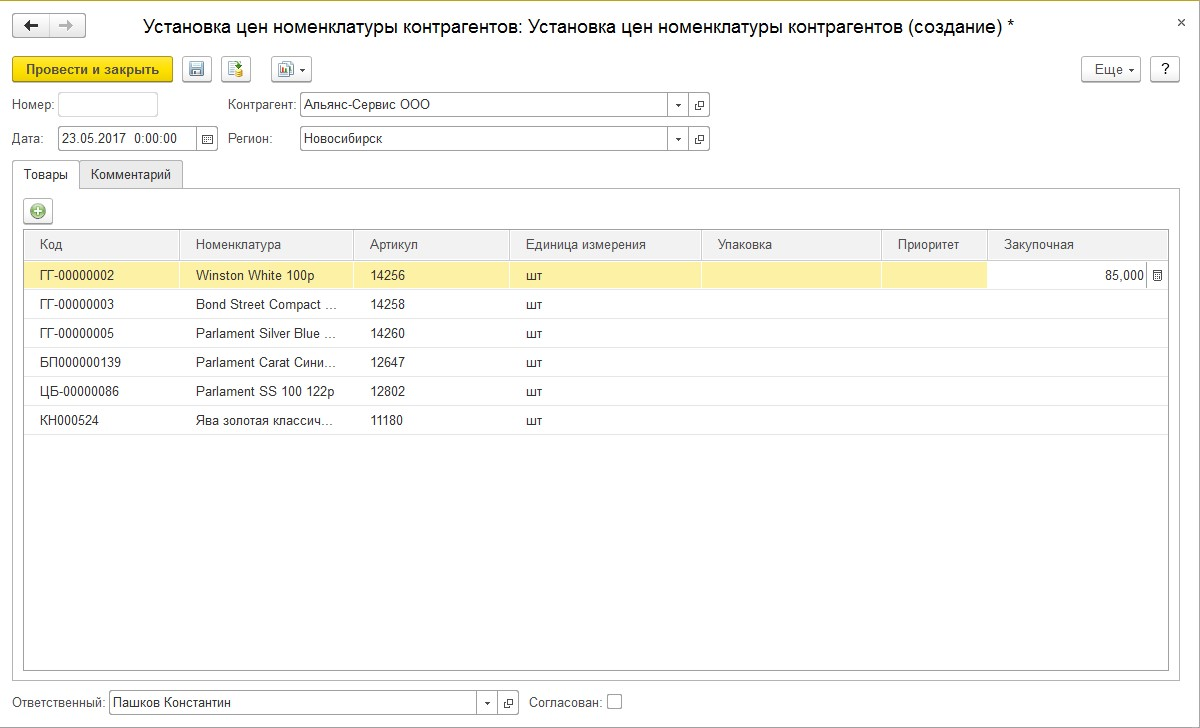
\includegraphics[width=0.8\textwidth]{26.jpg}
		 	\caption{Установка цен.}
		 	\label{ris:26.jpg}
		 \end{figure}		
		\item Также в документе для каждой позиции номенклатуры устанавливается "<Упаковка"> - минимальный объем, которым поставщик отгружает товар и есть возможность установить "<Приоритет"> поставщика для данной позиции. В дальнейшем приоритет будет использоваться при формировании заказов поставщикам при наличии нескольких поставщиков на одну позицию.
		\begin{figure}[H]
			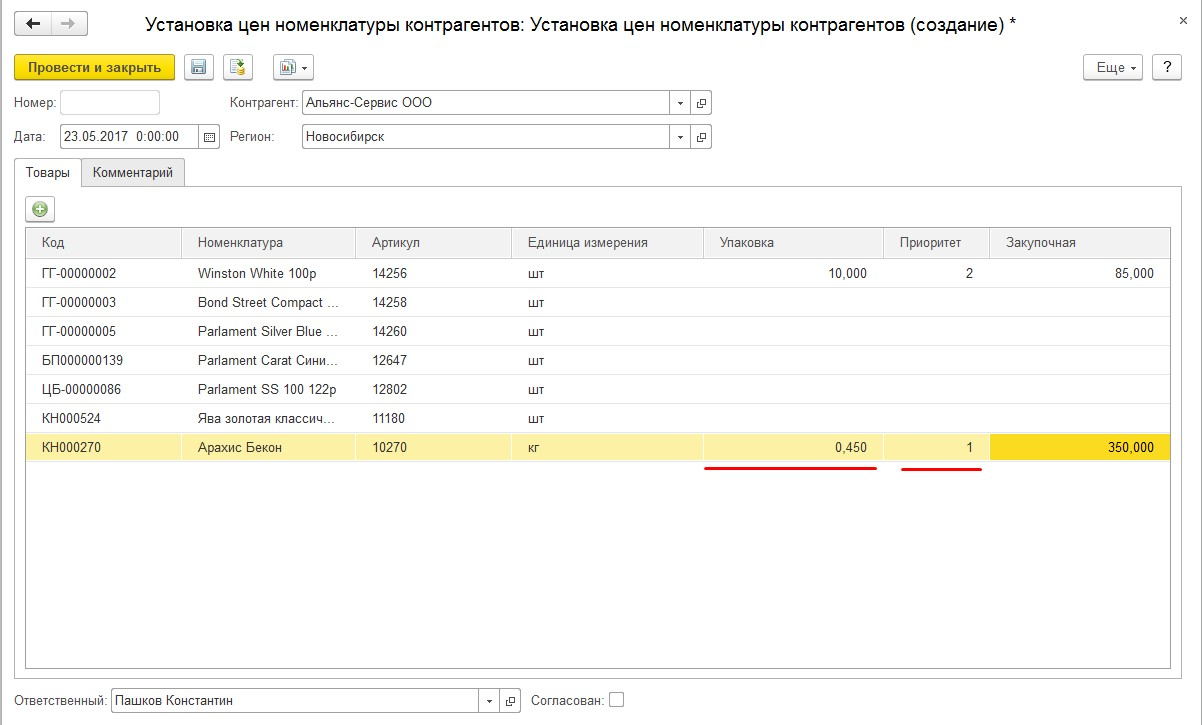
\includegraphics[width=0.8\textwidth]{31.jpg}
			\caption{Установка упаковки и приоритета.}
			\label{ris:31.jpg}
		\end{figure}			 
	 
 		\item Когда все цены заполнены документ можно провести \par используя кнопку 
\includegraphics[width=0.02\linewidth]{images/pr} ,,провести'' или \keys{Провести и закрыть}.
	\end{enumerate}	
	
%	\item Для добавления типа по конкретному поставщику, нужно из "<карточки"> контрагента открыть справочник "<Типы цен номенклатуры контрагентов"> как указано на Рис.~\ref{ris:14.jpg}
%	\item И с помощью кнопки "<Создать"> Добавить новый элемент
%	Рис.~\ref{ris:15.jpg}	
%	\begin{figure}[H]
%		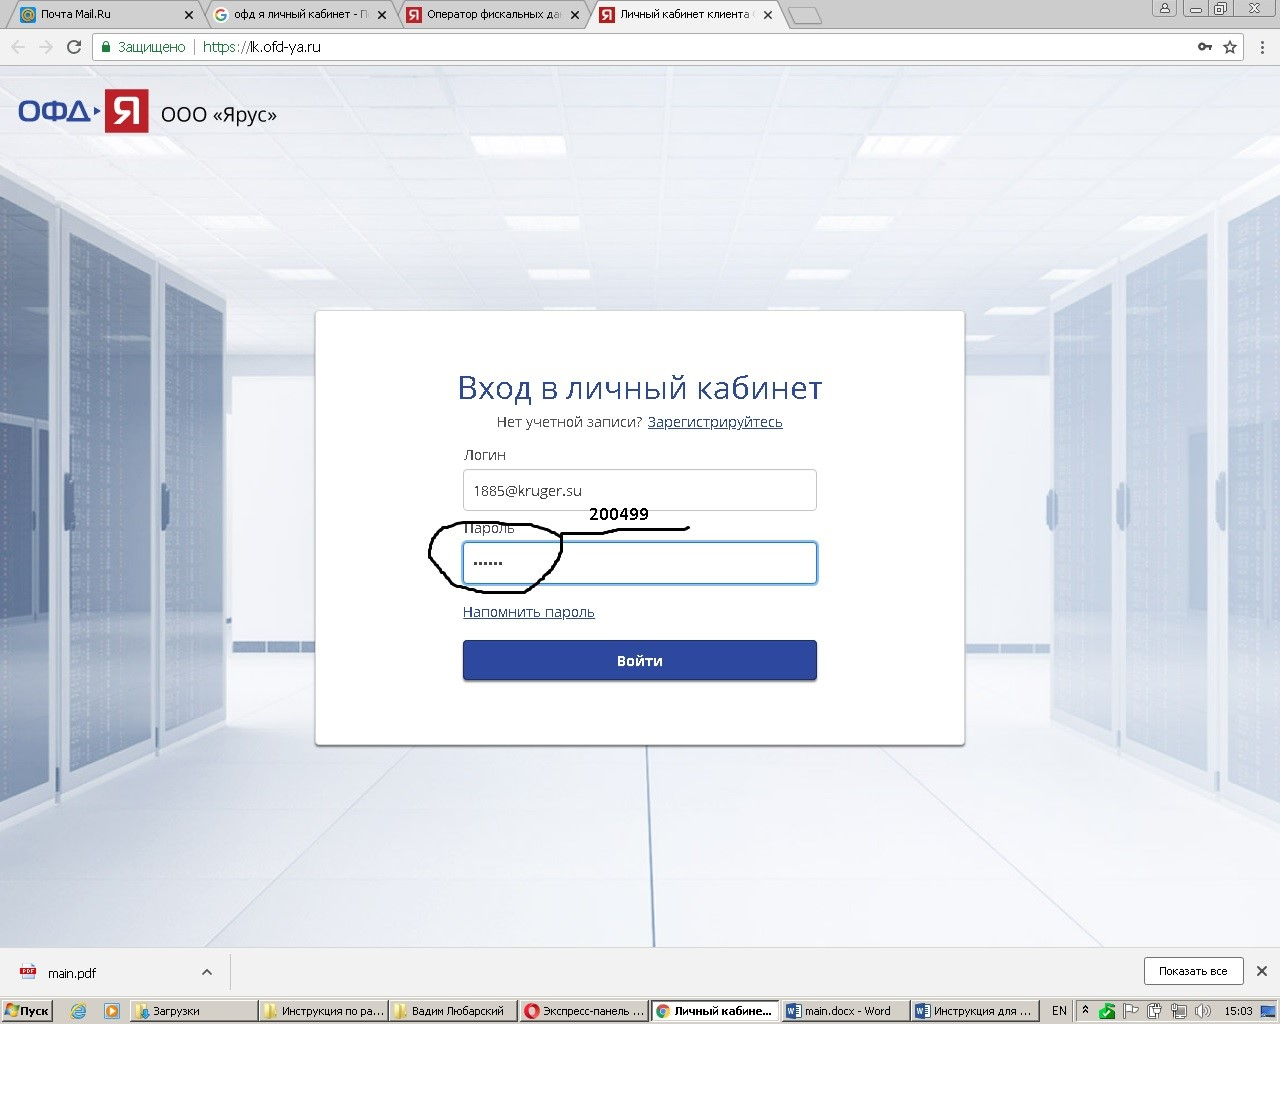
\includegraphics[width=0.7\textwidth]{15.jpg}
%		\caption{Создание нового элемента.}
%		\label{ris:15.jpg}
%	\end{figure}
%	\item Откроется форма создания нового элемента справочника "<Типы цен номенклатуры контрагентов"> Рис.~\ref{ris:16.jpg}
%	\begin{figure}[H]
%		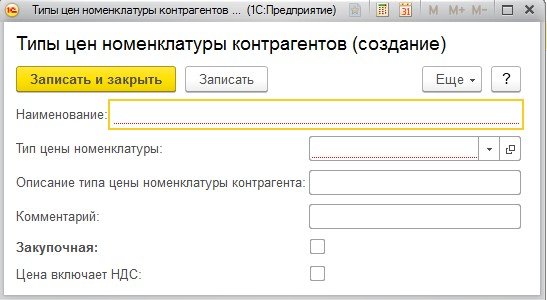
\includegraphics[width=0.7\textwidth]{16.jpg}
%		\caption{Новый элемент справочника.}
%		\label{ris:16.jpg}
%	\end{figure}  
%	
%	\item Необходимо заполнить данные для создания нового элемента справочника "<Типы цен номенклатуры контрагентов"> и  сохранить используя кнопку "<Записать и закрыть"> Рис.~\ref{ris:17.jpg}
%	\begin{figure}[H]
%		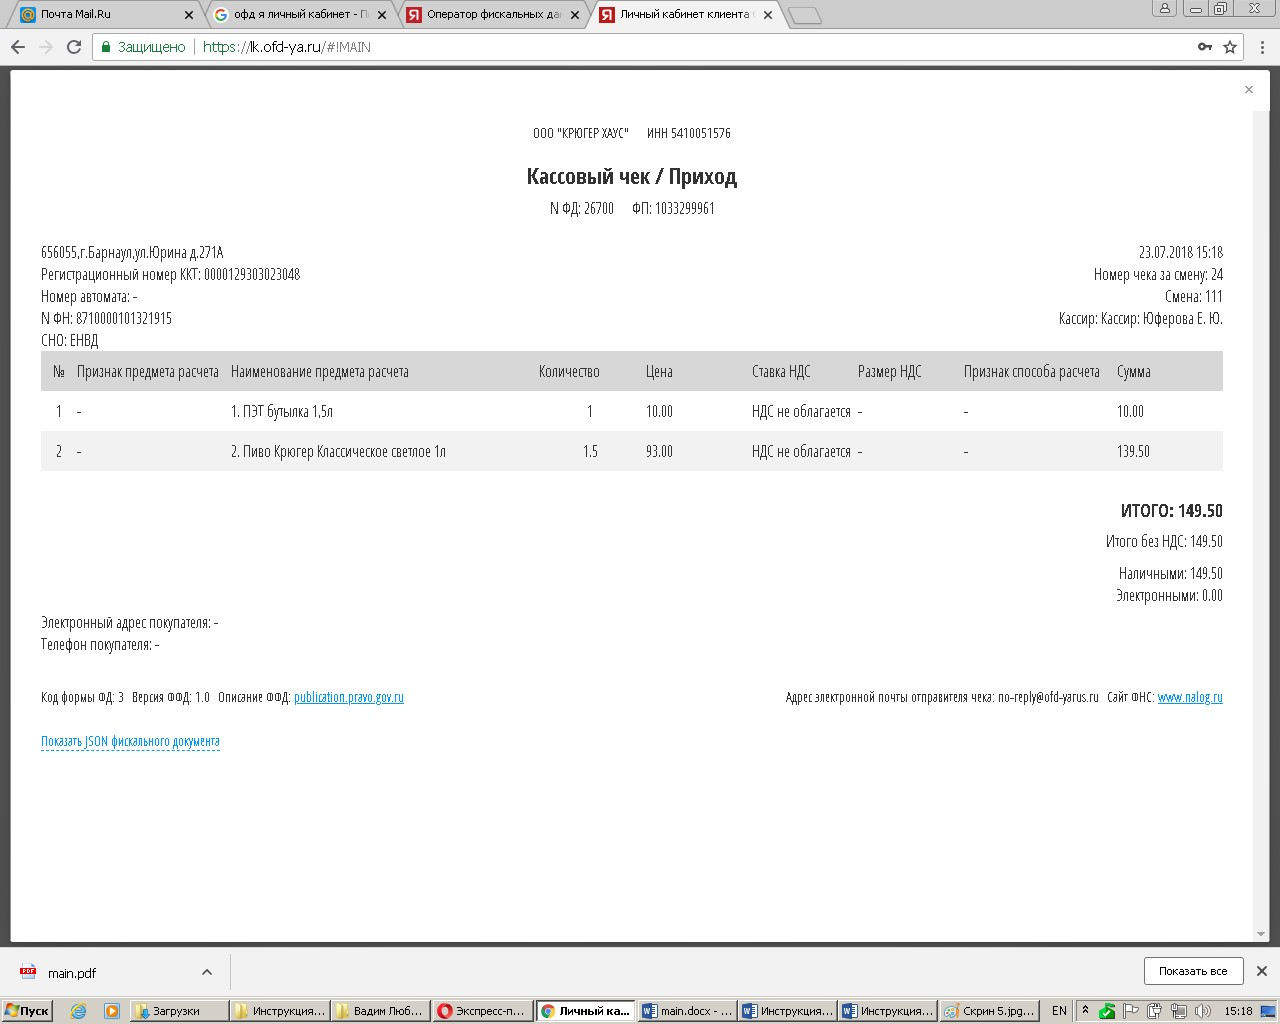
\includegraphics[width=0.7\textwidth]{17.jpg}
%		\caption{Заполненные данные.}
%		\label{ris:17.jpg}
%	\end{figure}  
%	
%	\item Появилась цена поставщика.  Рис.~\ref{ris:18.jpg}
%	Повторяем процедуру добавления, столько раз сколько цен у данного поставщика.
%	\begin{figure}[H]
%		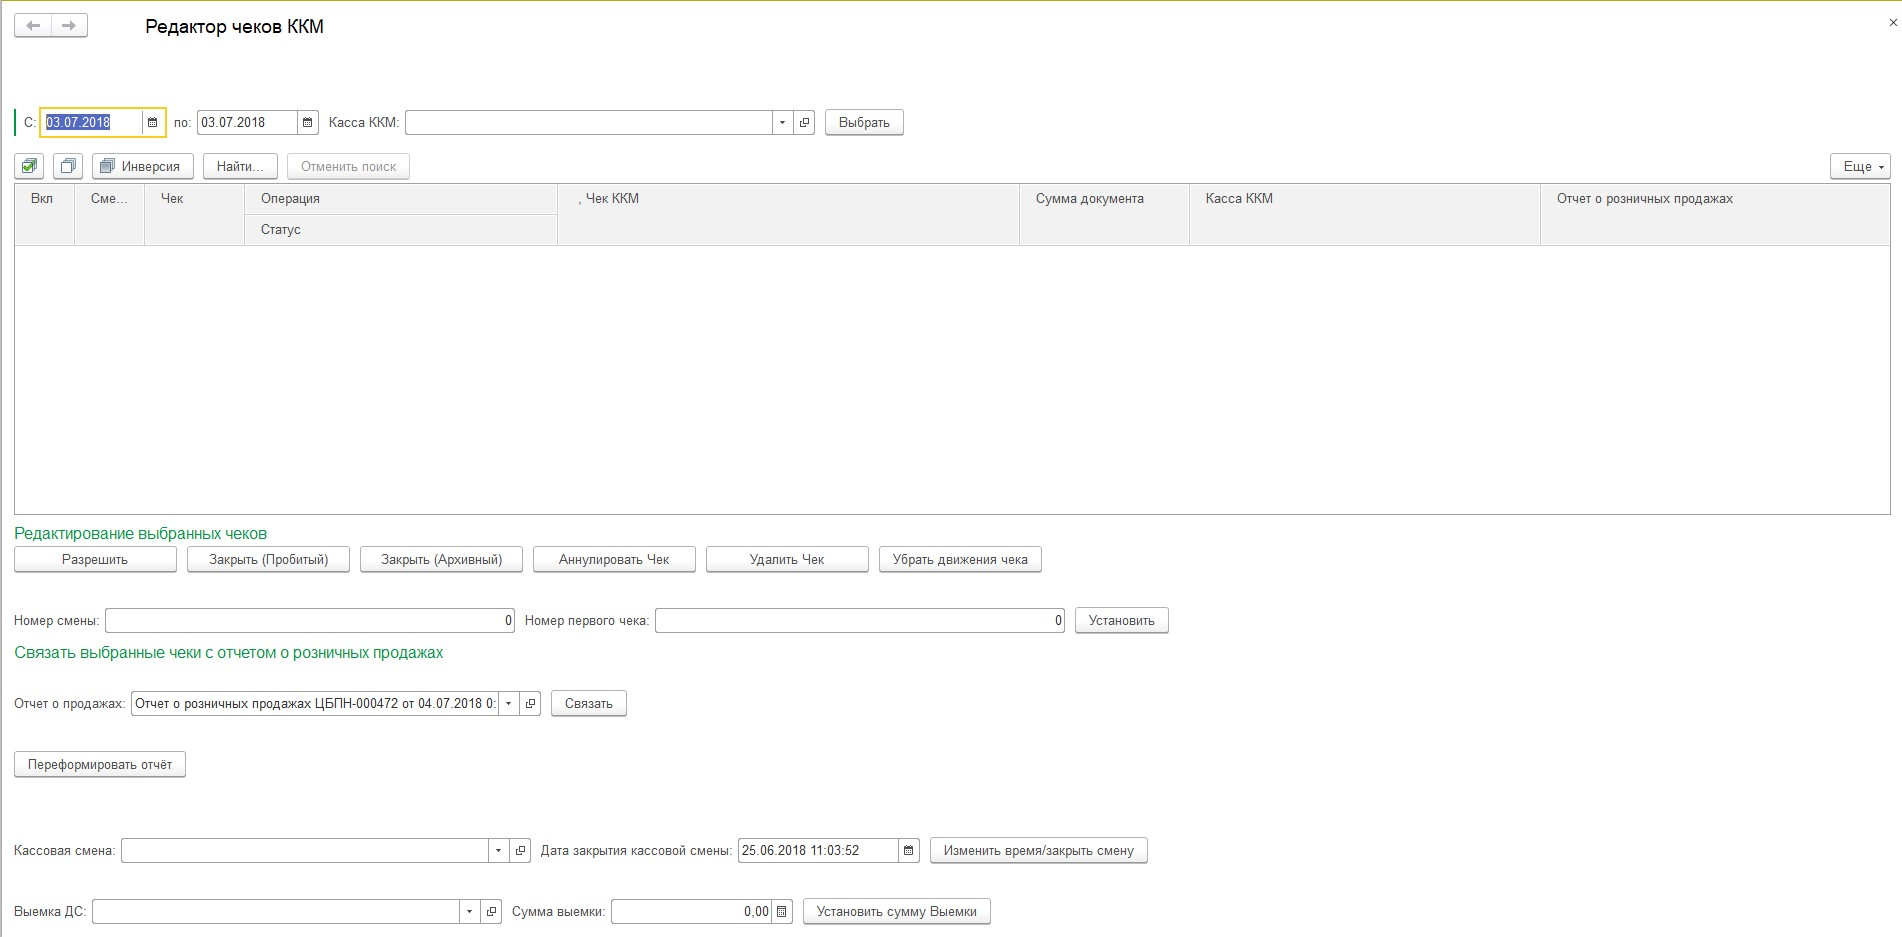
\includegraphics[width=0.7\textwidth]{18.jpg}
%		\caption{Добавлена цена.}
%		\label{ris:18.jpg}
%	\end{figure}  
%	
%	
	
\end{itemize}


